\FloatBarrier
\section[Fe-Pd Fit Parameters]{Iron-Palladium Potentials: Data and Initial Potential Parameters}

The developed code was used to fit a potential for Fe, Pd and their alloy.  A number of problems and limitations were encountered, and these will be discussed in more detail throughout this chapter and the conclusion.



\subsection{Bulk Properties for Fitting}

The fitting procedure is for both Fe and Pd, but the FCC allotrope of Fe that is used in this work does not exists, at room temperature and pressure.  Experimental data was available for Pd, but DFT generated data was required for Iron. 

\FloatBarrier
\subsubsection{Palladium [FCC]}

The input parameters for Pd are given in table \ref{table:pdinputparameters}. 

\begin{table}[ht]
\renewcommand{\arraystretch}{1.2}
\begin{tabular}{lccc}
\hline\hline
Property & \multicolumn{3}{c}{Value used in potential fitting} \\
\hline\hline
Element & \multicolumn{3}{c}{PD}\\
Structure             & \multicolumn{3}{c}{Face Centered Cubic}\\
$a_0$                 & \multicolumn{3}{c}{3.925 Angstrom \cite{webelementspd}}\\
Nearest Neighbour     & \multicolumn{3}{c}{ Angstrom \cite{webelementspd}}\\
Basis vectors         & $\begin{bmatrix} 1.0 & 0.0 & 0.0 \\ 0.0 & 1.0 & 0.0 \\ 0.0 & 0.0 & 1.0  \end{bmatrix}$ \\
$E_{coh}$             & \multicolumn{3}{c}{3.91 eV \cite{semiempiricalpots}}   \\
$B_0$                 & \multicolumn{3}{c}{184.4 GPA \cite{semiempiricalpots}}   \\
Elastic Constants     & $\begin{bmatrix} 218.5 & 151.4 & 151.4 & 0 & 0 & 0 \\ 151.4 & 218.5 & 151.4 & 0 & 0 & 0 \\ 151.4 & 151.4 & 218.5 & 0 & 0 & 0 \\ 0 & 0 & 0 & 80.3 & 0 & 0 \\ 0 & 0 & 0 & 0 & 80.3 & 0 \\ 0 & 0 & 0 & 0 & 0 & 80.3 \end{bmatrix}$ \\
\hline\hline
\end{tabular}
\caption{Pd input parameters for fitting}
\label{table:pdinputparameters}
\end{table}

\FloatBarrier
\subsubsection{Ruthenium [FCC]}

The input parameters for Ru are given in table \ref{table:ruinputparameters}. 

\begin{table}[ht]
\renewcommand{\arraystretch}{1.2}
\begin{tabular}{lccc}
\hline\hline
Property & \multicolumn{3}{c}{Value used in potential fitting} \\
\hline\hline
Element & \multicolumn{3}{c}{RU}\\
Structure             & \multicolumn{3}{c}{Face Centered Cubic}\\
$a_0$                 & \multicolumn{3}{c}{3.809 Angstrom \cite{webelementspd}}\\
Nearest Neighbour     & \multicolumn{3}{c}{ Angstrom \cite{webelementspd}}\\
Basis vectors         & $\begin{bmatrix} 1.0 & 0.0 & 0.0 \\ 0.0 & 1.0 & 0.0 \\ 0.0 & 0.0 & 1.0  \end{bmatrix}$ \\
$E_{coh}$             & \multicolumn{3}{c}{6.624 eV \cite{semiempiricalpots}}   \\
$B_0$                 & \multicolumn{3}{c}{307.8 GPA \cite{semiempiricalpots}}   \\
Elastic Constants     & $\begin{bmatrix} 471.5 & 219.1 & 219.1 & 0 & 0 & 0 \\ 219.1 & 471.5 & 219.1 & 0 & 0 & 0 \\ 219.1 & 219.1 & 471.5 & 0 & 0 & 0 \\ 0 & 0 & 0 & 245.0 & 0 & 0 \\ 0 & 0 & 0 & 0 & 245.0 & 0 \\ 0 & 0 & 0 & 0 & 0 & 245.0 \end{bmatrix}$ \\
\hline\hline
\end{tabular}
\caption{Pd input parameters for fitting}
\label{table:ruinputparameters}
\end{table}



\subsection{Bulk Properties for Fitting}





\FloatBarrier
\subsubsection{Iron [FCC]}


The input parameters were calculated by DFT, with an FCT structure rather than FCC, and the calculated bulk modulus, elastic constants and other related properties are in table \ref{table:feinputparameters}.

\begin{table}[ht]
\renewcommand{\arraystretch}{1.2}
\begin{tabular}{lccc}
\hline\hline
Property & \multicolumn{3}{c}{Value used in potential fitting} \\
\hline\hline
Element & \multicolumn{3}{c}{Fe}\\
Structure             & \multicolumn{3}{c}{Face Centered Cubic}\\
$a_0$                 & \multicolumn{3}{c}{3.59 Angstrom}\\
Nearest Neighbour     & \multicolumn{3}{c}{1.85 Angstrom}\\
Basis vectors         & $\begin{bmatrix} 0.96 & 0.0 & 0.0 \\ 0.0 & 1.00 & 0.0 \\ 0.0 & 0.0 & 0.96  \end{bmatrix}$ \\
$E_{coh}$             & \multicolumn{3}{c}{-4.32 eV}   \\
$B_0$ (GPA)           & \multicolumn{3}{c}{226.1}   \\
$E$ (GPA)             & \multicolumn{3}{c}{356.8}   \\
$G$ (GPA)             & \multicolumn{3}{c}{144.8}   \\
Poisson Ratio $\eta$  & \multicolumn{3}{c}{0.23}   \\
Elastic Constants     & $\begin{bmatrix} 364.6 & 141.6 & 233.8 & 0 & 0 & 0 \\ 141.6 & 298.7 & 130.4 & 0 & 0 & 0 \\ 233.8 & 130.4 & 364.6 & 0 & 0 & 0 \\ 0 & 0 & 0 & 186.3 & 0 & 0 \\ 0 & 0 & 0 & 0 & 266.8 & 0 \\ 0 & 0 & 0 & 0 & 0 & 186.3 \end{bmatrix}$ \\
\hline\hline
\end{tabular}
\caption{Fe input parameters for fitting}
\label{table:feinputparameters}
\end{table}

\FloatBarrier



\subsection{Reference Database}

A reference database of 72 configurations for Fe, 80 configurations for Pd and 152 combined for Fe-Pd was created using the DFT code PWscf.  This process and the python code used is detailed in section \ref{section:qeforfit}.




\FloatBarrier
\section{Iron-Palladium Potentials: First Potential}

The Fe potential consisted of a cubic knot-to-knot spline for the pair and density functions, and the Mendelev and Ackland type embedding functional as described in section \ref{section:prelimpotental}.  These functions were fit to the Sheng Pd plot to give the potential a starting point, and to ensure the density plot was a similar magnitude to the Pd potential that is also being derived, to give a reasonable starting point for the alloy fitting.

Similarly to the Fe potential, the Pd potential consisted of a cubic knot-to-knot spline were used for the pair and density with a 2 parameter embedding functional similar to that used by Mendelev and Ackland.  The Sheng Pd potentials were used as a starting point.  The parameters of the three functions were fit to the Sheng plots before then being fit to the \acrshort{dft} data and experimental bulk properties.

A total of 72 configurations were used in the fitting of Fe, but unfortunately only one of these had slightly randomised atomic positions.  This was due to an increase in SCF cycles and a number of convergence failures with the slightly perturbed atom positions.  The Pd potential was fit using the known experimental parameters and 80 \acrshort{dft} configurations, including 10 with randomised atom locations, slightly perturbed from the perfect crystal locations.  

Finally, the two already derived potentials (above) were combined.  A seventh potential was required to finish the potential, this being the Fe-Pd pair potential.  The Fe-Fe pair potential was used as a starting point.  All seven potentials were then fit to the Fe, Pd and Fe-Pd \acrshort{dft} configurations as well as both the Fe and Pd \acrshort{fcc} bulk properties.

Throughout, the simulated annealing and genetic algorithms were use in combination to optimise the potential parameters.  No local optimization methods were used with this potential.


\subsubsection{Fe-Pd Potential Properties}

The properties are calculated throughout the fitting process, but the final properties for both iron and Pd are presented in tables \ref{table:ironpotcalc} and \ref{table:palladiumpotcalc}.

\begin{table}[ht]
\renewcommand{\arraystretch}{1.2}
\begin{tabular}{lccc}
\hline\hline
Parameter & Experimental/DFT & This Potential & Error \%\\
\hline\hline
$a_0$ & 3.42   &  3.58  & 4.7\\
$e_0$ & -4.27  & -4.27 & 0.0 \\
$B_0$ & 222.0  &  238.8 & 7.6 \\
$C_{11}$ & 365.6  &  356.8 & 2.4 \\
$C_{22}$ & 298.7  &  296.1 & 0.9\\
$C_{33}$ & 364.0  &  356.8 & 2.0\\
$C_{44}$ & 186.3  &  180.9 & 2.9 \\
$C_{55}$ & 266.8  &  263.2 & 1.3 \\
$C_{66}$ & 186.3  &  180.9 & 2.9\\
$C_{12}$ & 141.6  &  139.1 & 1.8\\
$C_{13}$ & 233.8  &  241.7 & 3.4 \\
$C_{23}$ & 130.4  &  127.3 & 2.4 \\
\hline\hline
\end{tabular}
\caption{Experimental/dft properties for FCC iron vs those of the fe-pd potential}
\label{table:ironpotcalc}
\end{table}

\begin{table}[ht]
\renewcommand{\arraystretch}{1.2}
\begin{tabular}{lccc}
\hline\hline
Parameter & Experimental/DFT & This Potential & Error \%\\
\hline\hline
$a_0$ & 3.89 & 3.95  & 1.5\\
$e_0$ & -3.91  & -3.91  & 0.0 \\
$B_0$ & 180.0  & 171.3 & 4.8 \\
$C_{11}$ & 234.0  & 248.9 & 6.4 \\
$C_{12}$ & 176.0  & 167.2 & 5.0 \\
$C_{44}$ & 71.2  & 67.6 & 5.1 \\
\hline\hline
\end{tabular}
\caption{Experimental/dft properties for FCC palladium vs those of the fe-pd potential}
\label{table:palladiumpotcalc}
\end{table}

\FloatBarrier
\subsubsection{Fe-Pd Property Plots}

The equation of state and elastic constants were used to fit the potential, and for both iron and palladium the fit reasonable well.  The data points produced for the Fe \acrshort{eos} do curve down slightly more that might be expected, but the data points for the Pd \acrshort{eos} do better fit the curve of the equation of state (appendix \ref{section:fepdv1eosec}).

To test the cohesive energy a short python code was written to generate 4x4x4 \acrshort{fcc} supercells with a lattice parameter ranging 9.58 angs to 36.9 angs for iron and 10.9 angs to 42.0 angs for palladium.  An energy calculation was performed for each element, using the derived potential, and the results were plotted (appendix \ref{section:fepdv1coh}, figs. \ref{fig:fev1cohesive}, \ref{fig:fev1cohesivezoom}, {fig:pdv1cohesive}, \ref{fig:pdv1cohesivezoom}).

The cohesive energy plots for both iron and palladium take on a recognisable shape and, over all they do give the predicted cohesive energies.  Neither is very smooth and to improve the reproduction of the correct energy at varying lattice parameters the energies should be computed using \acrshort{dft} and used during the potential fit.

The surface energies were also calculated.  A small python program was created to generate a set of 4x4x4 \acrshort{fcc} atoms.  The position and separation of the atoms was fixed relative to one another, and anchored to the 0,0,0 coordinate, whilst the unit vector in the z axis was increased.  This represents the transition from a bulk material to a slab with two surfaces in the xy-plane.

\begin{equation}
\begin{split}
E_s = \frac{E_{total} - N_a \times E_{bulk}}{2A_{surface}} \\
\text{where } E_s = \text{ surface energy} \\
\text{and } E_{total} = \text{ total energy of slab} \\
\text{and } N_a = \text{ atoms in bulk} \\
\text{and } E_{bulk} = \text{ atom energy in bulk} \\
\text{and } A_{surface} = \text{ surface area of slab in xy-plane} \\
\end{split}
\label{eq:newspline}
\end{equation}

The calculated surface energies were $0.205eV/ang^2$ ($3,290 mJ/m^2$) for iron and for $0.106eV/ang^2$ ($1690 mJ/m^2$) palladium.  The plots for these calculations are in appendix \ref{section:fepdv1se} (figs. \ref{fev1surface}, \ref{pdv1surface}).  Whilst the value for palladium is close to the experimental and Sheng values, ($2,000 mJ/m^2$ and $1,747 mJ/m^2$ respectively \cite{shengeamonline}), the calculations were performed without relaxing the atoms at each stage.  This will be discussed further in chapter \ref{chapter:futurework}.





\FloatBarrier
\section{Iron-Palladium Potentials: Second Potential}

A second attempt was made to derive an iron-palladium and several changes were made.  First, the neighbour separations were examined for both palladium and iron, as shown in fig. \ref{fig:fcc-fe-neighbours} and fig. \ref{fig:fcc-pd-neighbours}.  Knot-to-knot splines offer a high degree of flexibility, but there is a problem.  If the movement of one, or more, knots does not have a direct effect on any of the bulk property or energy, stress, force calculations it will move during optimization resulting in what looks to be a very badly behaved function.  It also unnecessarily increases the parameter space for optimization.

\begin{figure}[htp]
  \begin{center}
    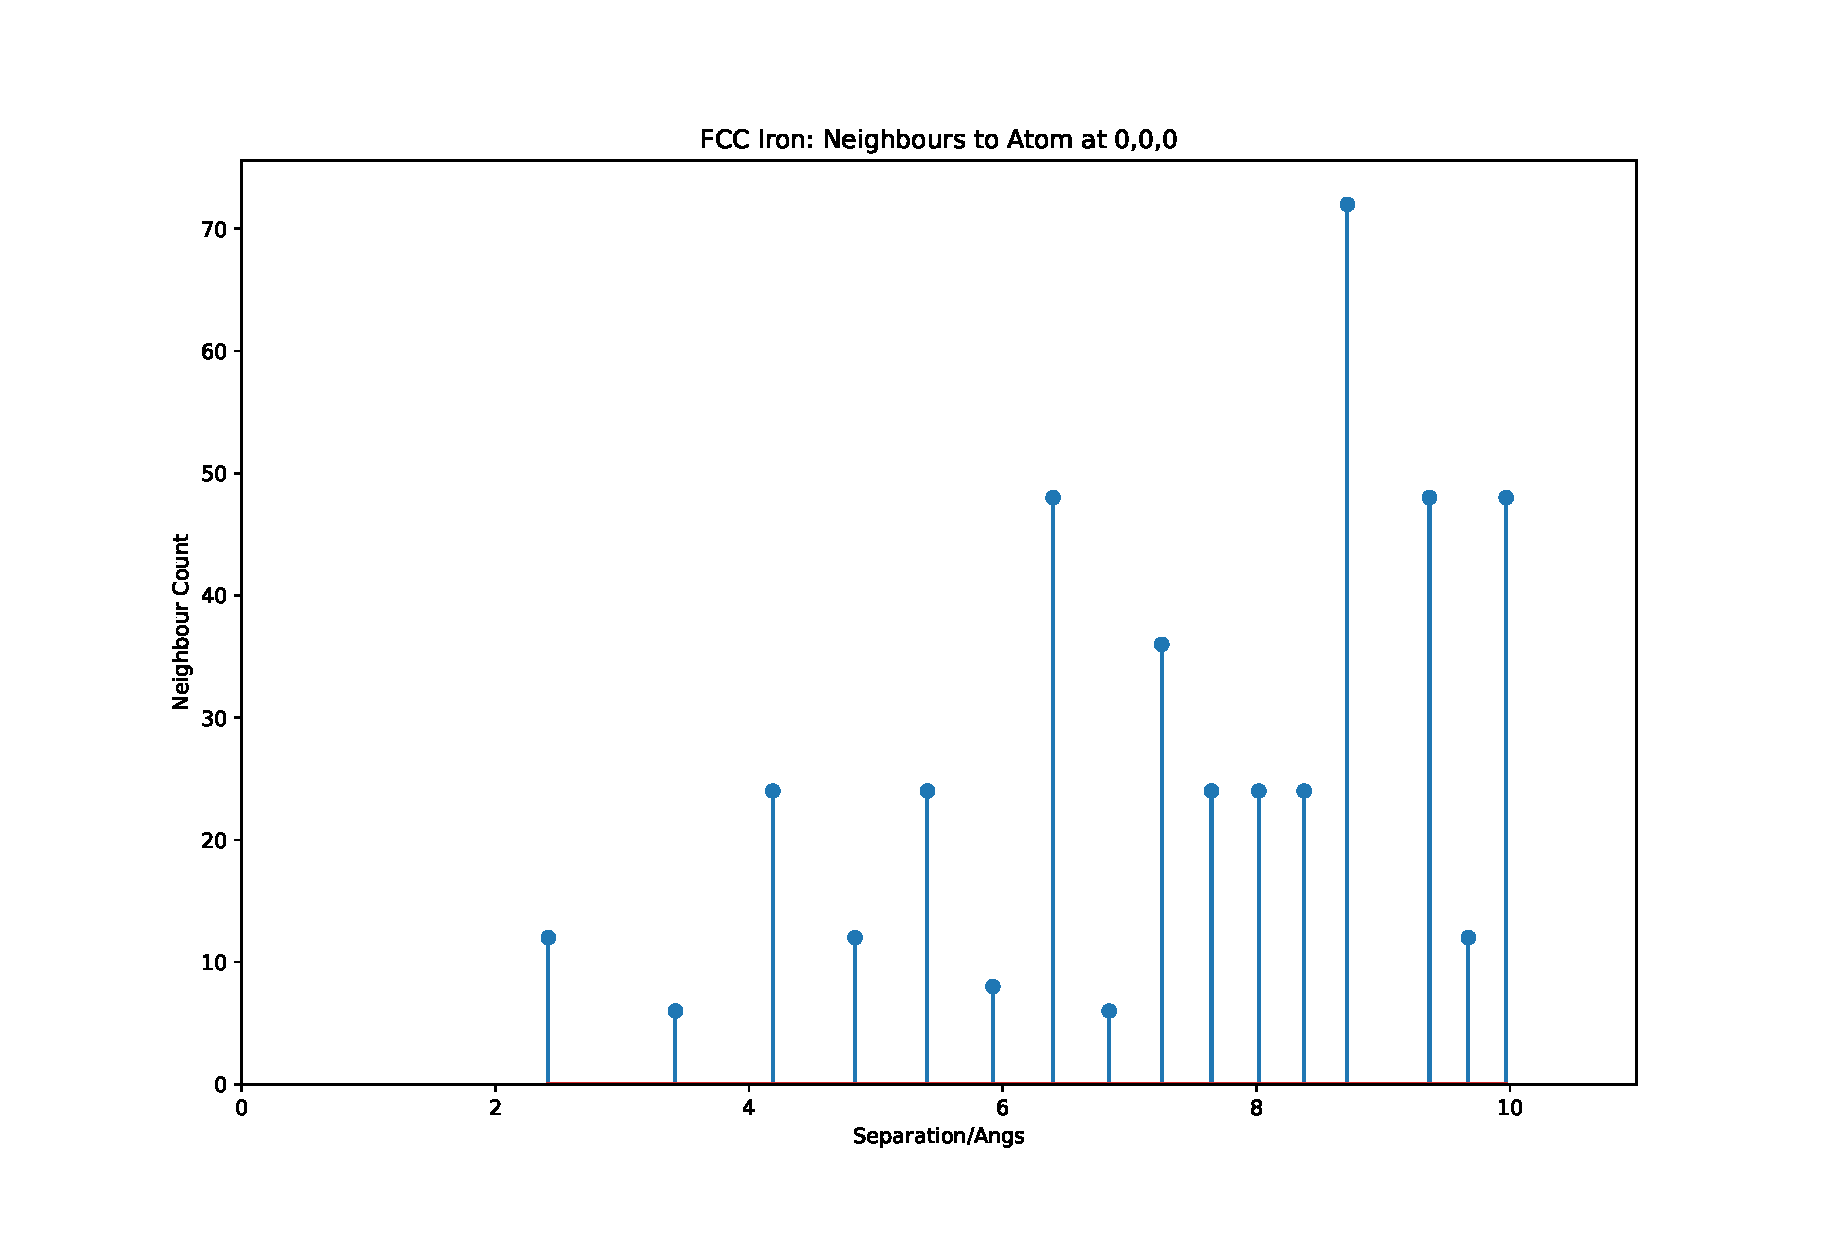
\includegraphics[scale=0.55]{chapters/results_potential_fitting/neighbours/fe.eps}
    \caption{FCC Iron Neighbour Separation}
    \label{fig:fcc-fe-neighbours}
  \end{center}
\end{figure}

\begin{figure}[htp]
  \begin{center}
    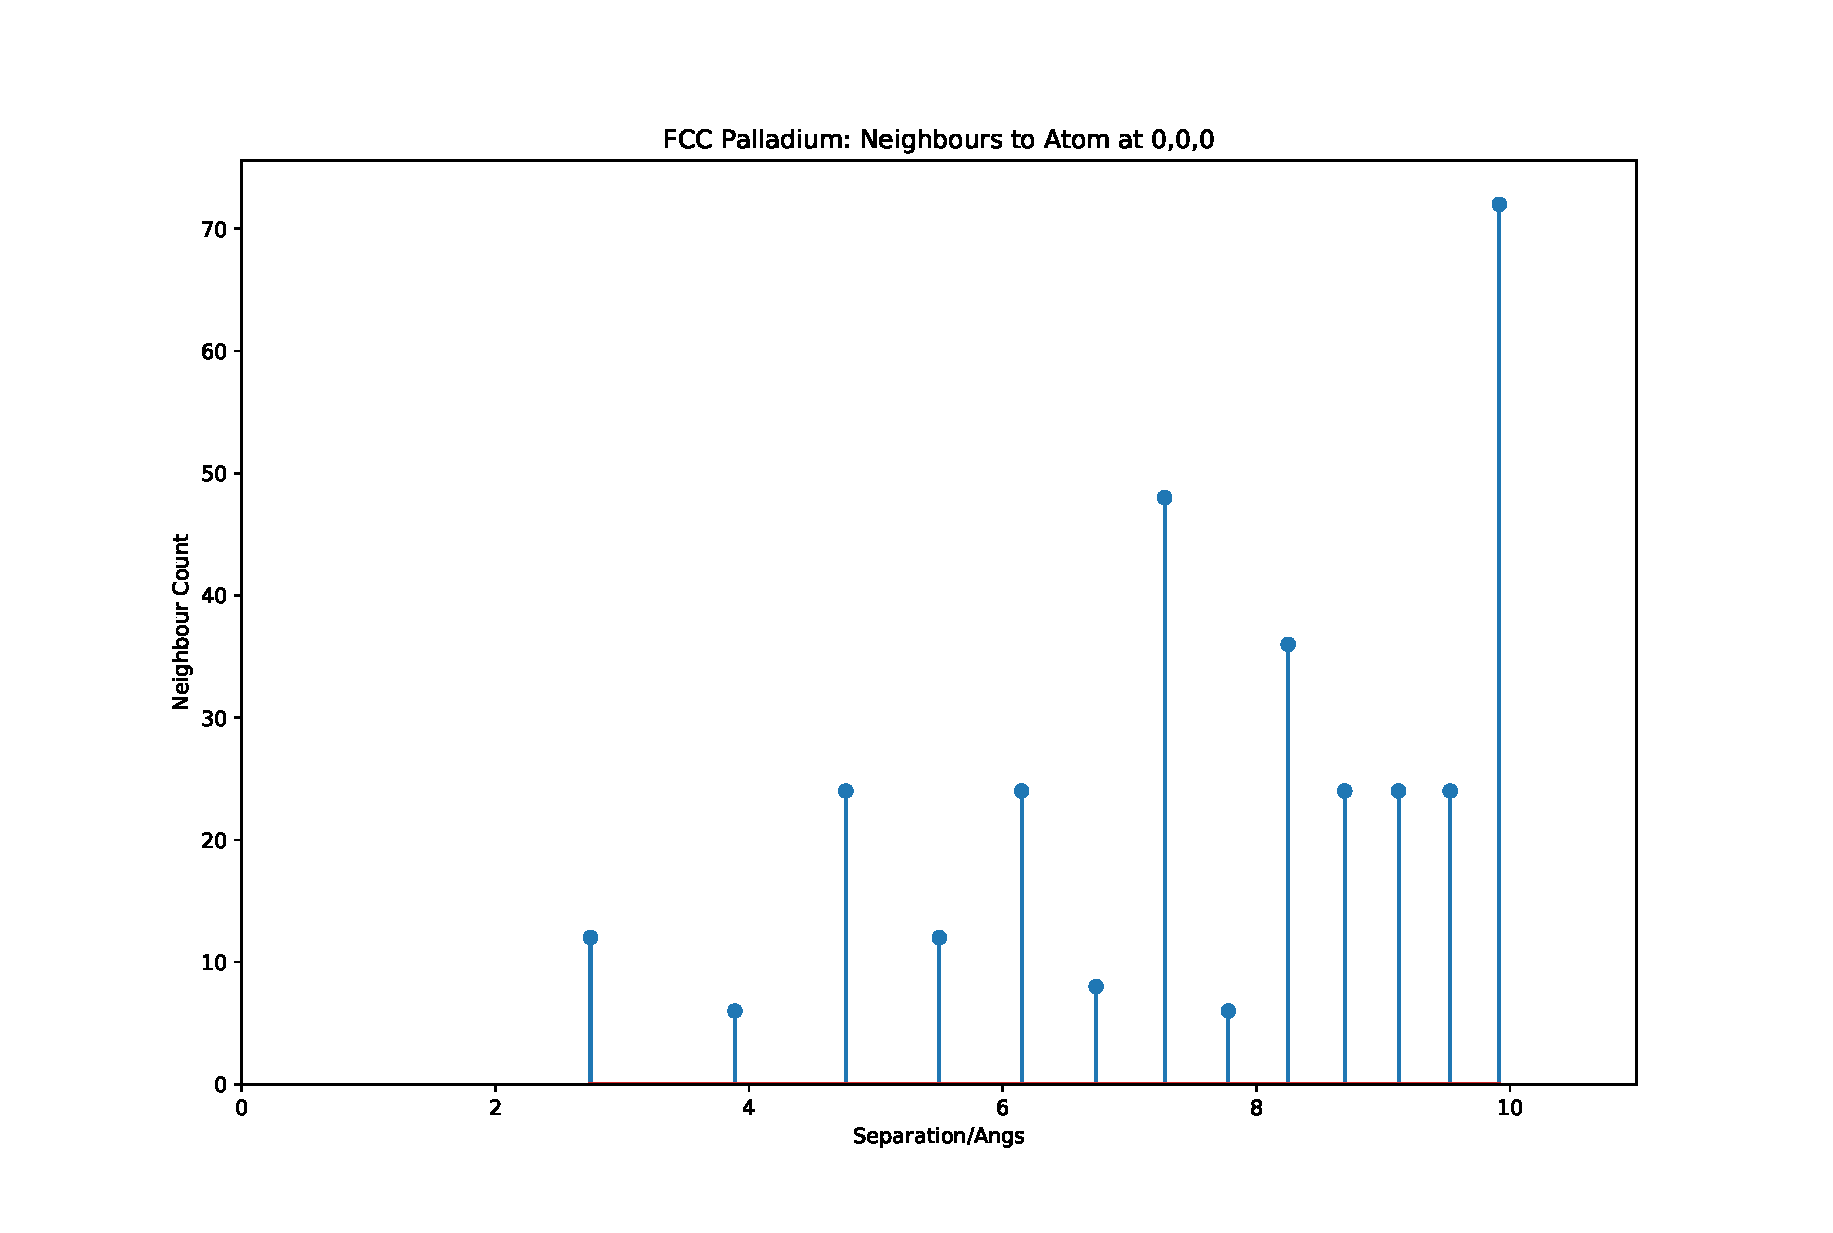
\includegraphics[scale=0.55]{chapters/results_potential_fitting/neighbours/pd.eps}
    \caption{FCC Palladium Neighbour Separation}
    \label{fig:fcc-pd-neighbours}
  \end{center}
\end{figure}

The number of knots for the pair functions was reduced to 7, including the start and end knot.  This would help reduce the number of superfluous knots, decreasing the parameter space, with the aim of also ending with a smoother function.  A major change was also made to the cubic knot function.  The entire function would be the \acrshort{zbl} potential summed with a cubic knot spline, to give a function with a continuous value and derivative (eq. \ref{eq:newspline}).

\begin{equation}
\begin{split}
v(r) = zbl(r, z_a, z_b) + spline(r, \vec{p})
\end{split}
\label{eq:newspline}
\end{equation}

Another change implemented was to the way the parameters for the cubic knot spline functioned.  Originally, the x positions for the knots were set by the user and the y positions were varied by the fitting program.  The derivative at each point, needed to calculate each knot to knot spline, was interpolated.  In the latest version the user specifies x, y(x) and y'(x) for the end knot (in this work, 6.5 0.0 and 0.0) and the x value of the start knot (in this work, 0.0).  The remaining x, y(x) and y'(x) are all parameters that are varied by the fitting code.

The spline used previously for the density function was replaced with a 2 parameter Slater type function.  The embedding functional remained the same.  The starting potentials for both iron and palladium were fit to the Sheng potential for palladium and the same bulk properties and \acrshort{dft} configurations were used as for the first potential.

The fitting code was modified to include the SciPy optimization library.  As a result, the potentials were fit using the simulated annealing and genetic algorithm for global optimisation, then Nelder-Mead and \acrlong{bfgs} to optimise the parameters locally.




\FloatBarrier
\subsubsection{Fe-Pd Calculated Properties}

The properties are calculated throughout the fitting process, but the final values for both Fe and Pd are presented in tables \ref{table:ironpotcalc2} and \ref{table:palladiumpotcalc2}.

\begin{table}[ht]
\renewcommand{\arraystretch}{1.2}
\begin{tabular}{lccc}
\hline\hline
Parameter & Experimental/DFT & This Potential & Error \%\\
\hline\hline
$a_0$ & 3.42   &  3.40 & 0.6 \\
$e_0$ & -4.27  & -4.29 & 0.5 \\
$B_0$ & 222.0  &  229.1 & 3.5 \\
$C_{11}$ & 365.6  &  365.9 & 0.1\\
$C_{22}$ & 298.7  &  298.6 & 0.0 \\
$C_{33}$ & 364.0  &  365.9 & 0.5\\
$C_{44}$ & 186.3  &  187.6 & 0.7 \\
$C_{55}$ & 266.8  &  258.4 & 3.1 \\
$C_{66}$ & 186.3  &  187.6 & 0.7 \\
$C_{12}$ & 141.6  &  141.1 & 0.4 \\
$C_{13}$ & 233.8  &  238.1 & 1.8 \\
$C_{23}$ & 130.4  &  124.8 & 4.3 \\
\hline\hline
\end{tabular}
\caption{Experimental/dft properties for FCC iron vs those of the fe-pd potential}
\label{table:ironpotcalc2}
\end{table}

\begin{table}[ht]
\renewcommand{\arraystretch}{1.2}
\begin{tabular}{lccc}
\hline\hline
Parameter & Experimental/DFT & This Potential & Error \%\\
\hline\hline
$a_0$ & 3.89 & 3.87 & 0.5 \\
$e_0$ & -3.91  & -3.91 & 0.0 \\
$B_0$ & 180.0  & 171.3 & 4.8 \\
$C_{11}$ & 234.0  & 232.9 & 0.5 \\
$C_{12}$ & 176.0  & 176.7 & 0.4 \\
$C_{44}$ & 71.2  & 68.8 & 3.4 \\
\hline\hline
\end{tabular}
\caption{Experimental/dft properties for FCC palladium vs those of the fe-pd potential}
\label{table:palladiumpotcalc2}
\end{table}

\FloatBarrier
\subsubsection{Fe-Pd Property Plots}

The equation of state and elastic constants were used to fit the potential, and for both iron and palladium they fit reasonable well.  The largest error is for the bulk modulus of Pd with a value 4.8\% less than the actual bulk modulus.

The cohesive energies were calculated similarly to the first version, using the prepared configurations to expand the cell until the atoms are isolated from their neighbours.  The energies were plotted at various values of lattice parameter (appendix \ref{section:fepdv2coh} figs. \ref{fig:fev2cohesive}, \ref{fig:fev2cohesivezoom}, {fig:pdv2cohesive}, \ref{fig:pdv2cohesivezoom}).  Both the Fe and Pd plots are quite poor with a smooth but erratic trend in data points with a sharp drop for the largest value of $a_0$.  This supports using \acrshort{dft} data to accurately calculate the cohesive energy plot data points and use these in the potential fitting process.


The calculated surface energies were $0.506eV/ang^2$ ($8,110 mJ/m^2$) for iron and for $0.058eV/ang^2$ ($932 mJ/m^2$) palladium.  The energy for palladium is under half that expected.  The value for iron in comparison is rather large, but the surface energy for \acrshort{fcc} iron would need to be calculated using \acrshort{dft} to determine whether or not it is a sane value or not.  The plots for the surface energy calculations are contained in appendix \ref{section:fepdv2se} (figs. \ref{fev2surface}, \ref{pdv2surface}).



\FloatBarrier







%%%%%%%%%%%%%%%%%%%%%%%%%%%%%%%%%%%%%%%%%%%%%%%%%%%%%%%%%%%%%%%%%%%%%%%%%%%%%%%%%%%%%%%%%%%%%%%%%%%%%%%%%%
%%
%%  Results DFT Database
%%  
%%%%%%%%%%%%%%%%%%%%%%%%%%%%%%%%%%%%%%%%%%%%%%%%%%%%%%%%%%%%%%%%%%%%%%%%%%%%%%%%%%%%%%%%%%%%%%%%%%%%%%%%%%



\FloatBarrier
\section{DFT Configuration Database}
\label{section:dftconfigurationdbresults}




\begin{figure}[htb]
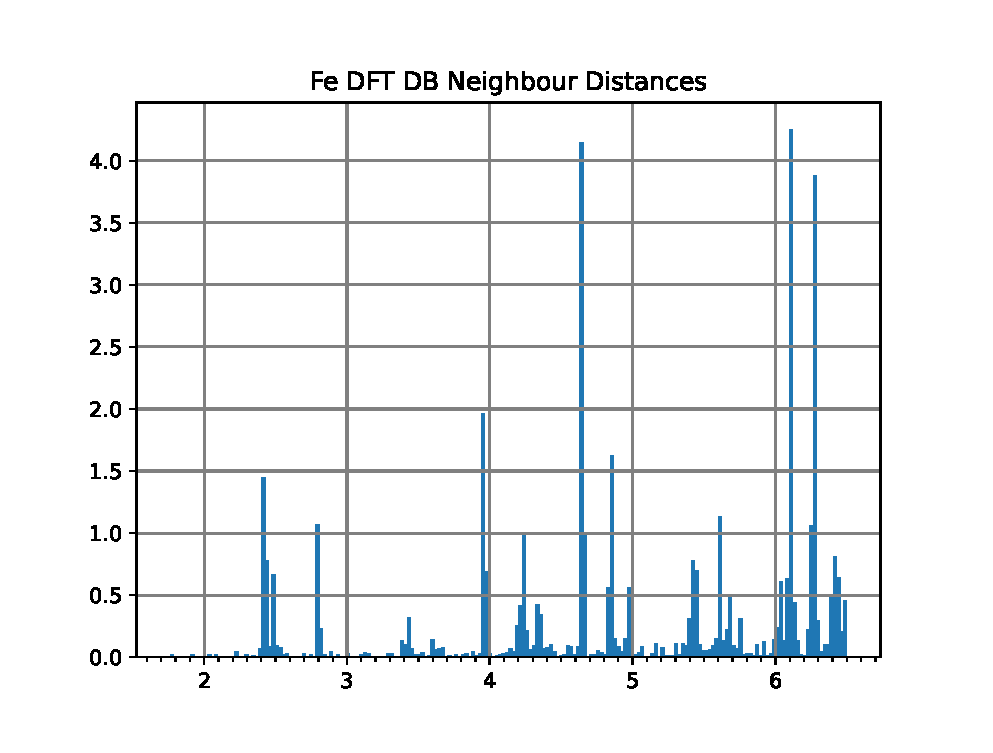
\includegraphics[width=0.5\linewidth]{chapters/results_dft_reference_db/neighbour_distances/db_fe_neighbours.eps}
\caption{Iron Database Neighbour Separation Distances}
\label{fig:shengpdpair}
\end{figure}


\begin{figure}[htb]
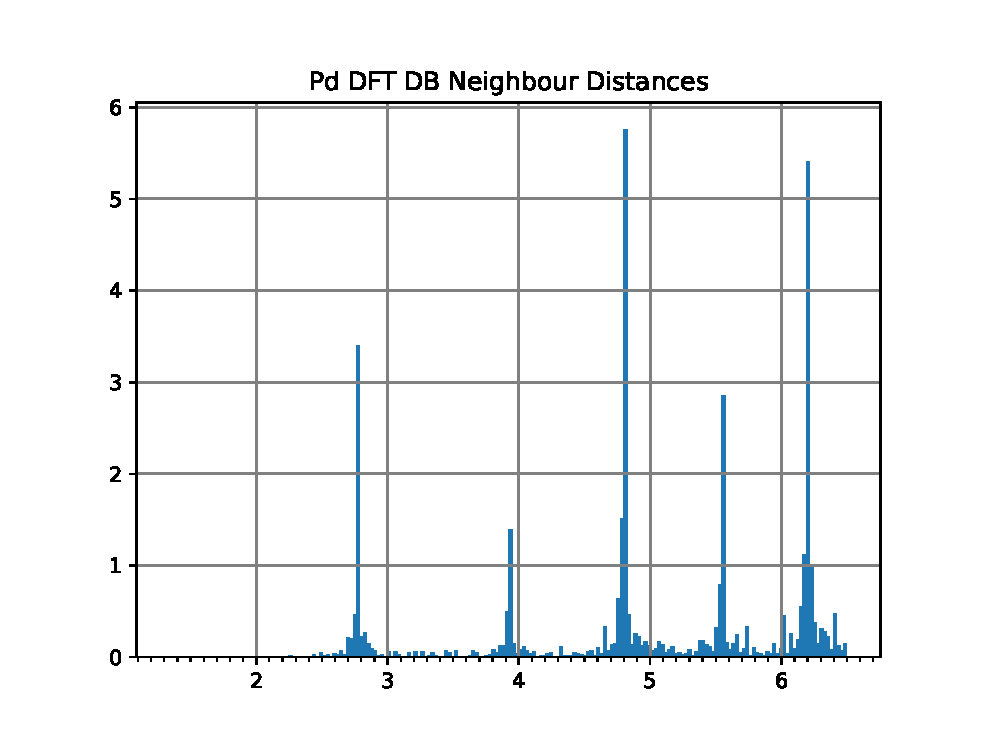
\includegraphics[width=0.5\linewidth]{chapters/results_dft_reference_db/neighbour_distances/db_pd_neighbours.eps}
\caption{Palladium Database Neighbour Separation Distances}
\label{fig:shengpdpair}
\end{figure}


\begin{figure}[htb]
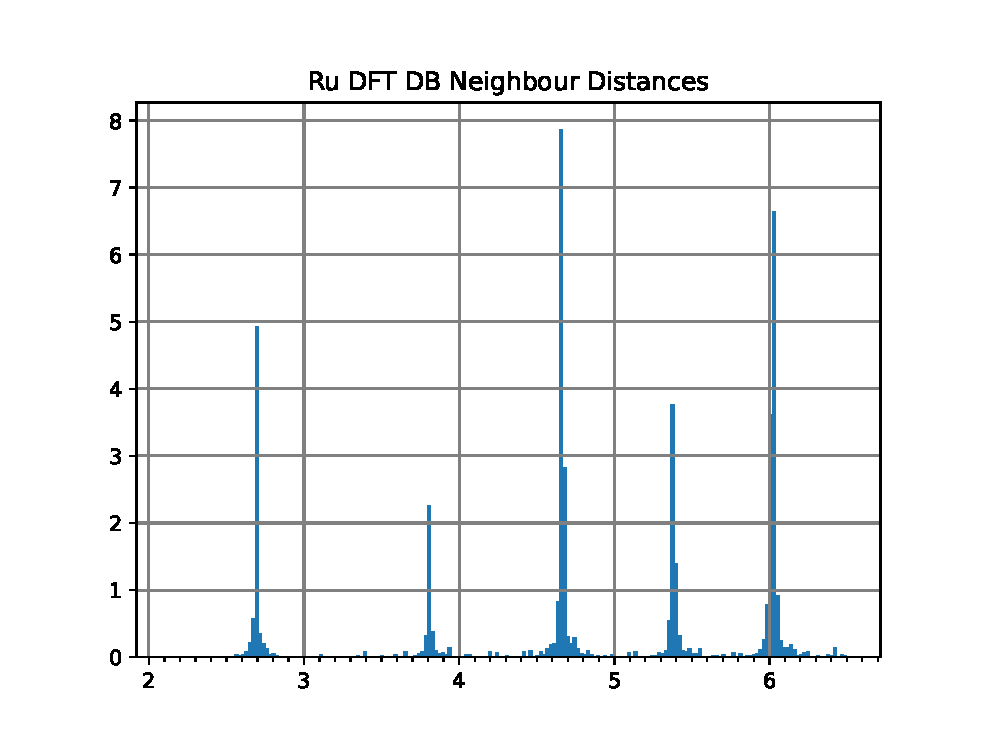
\includegraphics[width=0.5\linewidth]{chapters/results_dft_reference_db/neighbour_distances/db_ru_neighbours.eps}
\caption{Ruthenium Database Neighbour Separation Distances}
\label{fig:shengpdpair}
\end{figure}



\begin{figure}[htb]
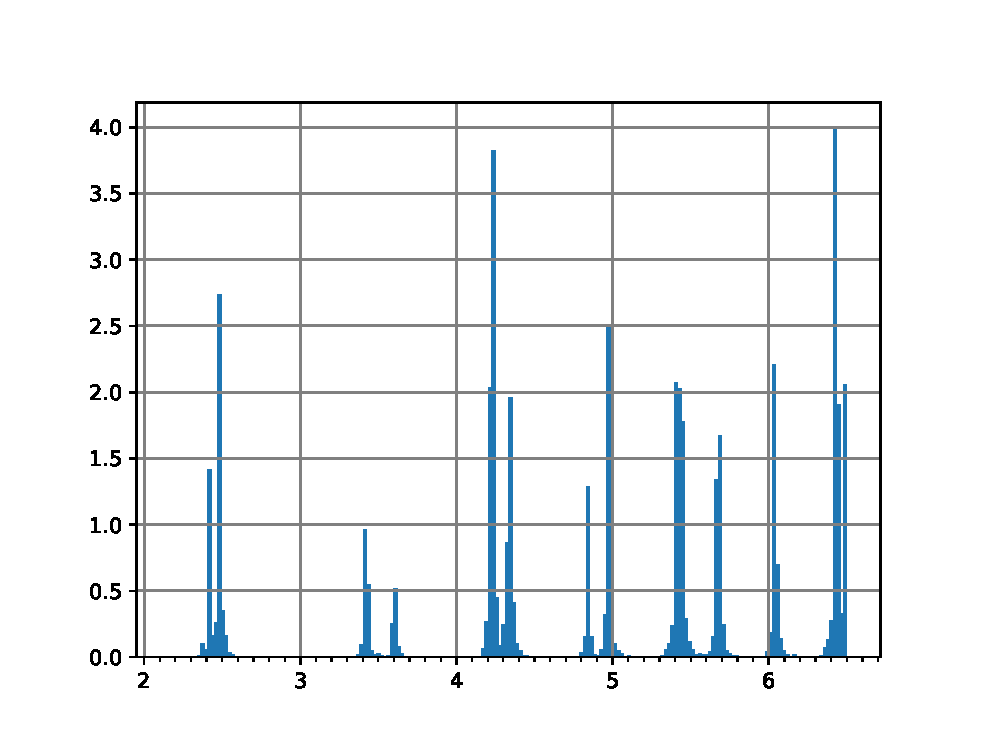
\includegraphics[width=0.5\linewidth]{chapters/results_dft_reference_db/neighbour_distances/db_feru_neighbours.eps}
\caption{Iron Database Neighbour Separation Distances}
\label{fig:shengpdpair}
\end{figure}


\begin{figure}[htb]
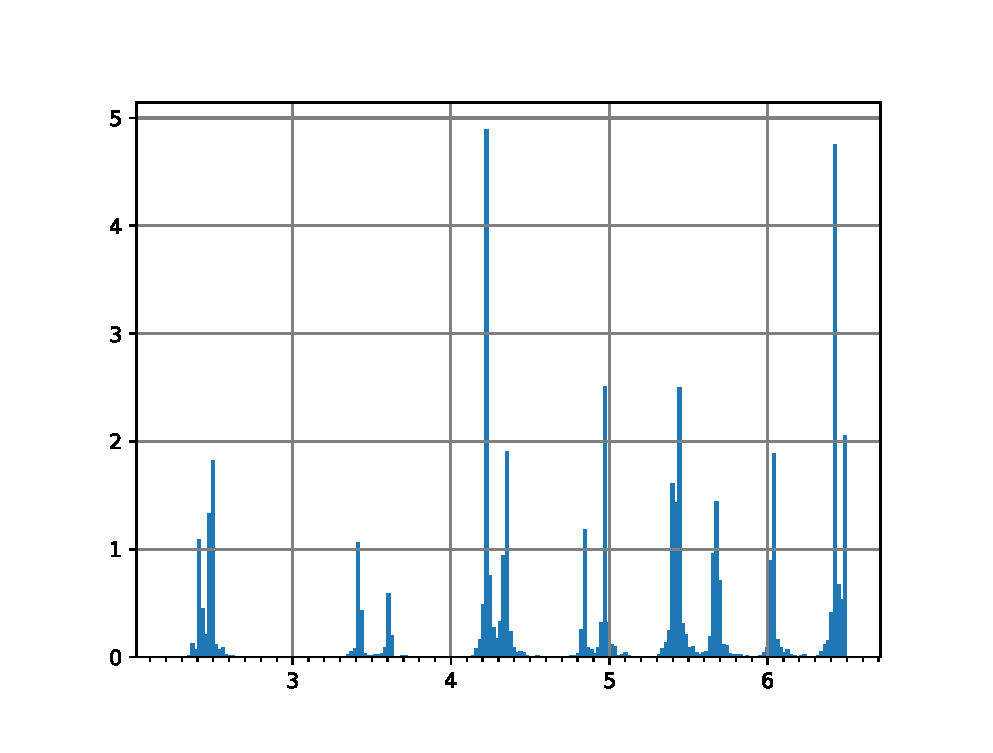
\includegraphics[width=0.5\linewidth]{chapters/results_dft_reference_db/neighbour_distances/db_fepd_neighbours.eps}
\caption{Iron Database Neighbour Separation Distances}
\label{fig:shengpdpair}
\end{figure}


\subsection{Calibrating the Database Energies}

There energies computed with \acrshort{dft} are not equivalent to known energies, such as the cohesive energy.  The actual energies may be determined either using the known cohesive energy of the relaxed material or by using the isolated atom energies computed with \acrshort{dft}, that would have a zero energy.

\begin{table}[h]
\begin{center}
\begin{tabular}{c c c c c c}
\hline\hline
Element & Structure & Atoms  & Relaxed per Atom (Ry) & Known Cohesive Energy (eV) & Offset (eV)\\
\hline\hline
Fe      & BCC       & 32     & -329.2618197          & -4.316               & 4475.519239  \\
Ru      & HCP       & 16     & -431.6742014          & -6.74                & 5866.486665  \\
Pd      & HCP       & 16     & -512.0299524          & -3.91                & 6962.612344  \\
Fe      & BCC       & 128     & -329.2578402          & -4.316               & 4475.465095  \\
Ru      & HCP       & 256     & -431.6697631          & -6.74                & 5866.426278  \\
Pd      & HCP       & 128     & -512.0277034          & -3.91                & 6962.581745  \\
\hline\hline
\end{tabular}
\end{center}
\caption{Offset energies computed for 16/32 and 128/256 atom configurations}
\label{table:dftoffsetenergies}
\end{table}

To preserve the known cohesive energy the first method was used.  The relaxed configuration of 32 atoms and 128 atoms was computed for each element.  The was evaluated along with the cohesive energy for each to give an offset to be applied to all calculations on an atom by atom basis.

All the configurations used in the reference database are process and the \acrshort{dft} energies are recalculated atom by atom with the offsets applied.  Those with 16-32 atoms have the first set of offsets applied, whereas larger configurations using the Gamma k-point have the second set of offsets applied.


\subsection{Cohesive Energy Configurations}





\subsection{Surface Energy and Slabs}



\subsection{Defect Calculation}


\subsection{Equation of State and Elastic Constant Configurations}


